\documentclass[
11pt, % The default document font size, options: 10pt, 11pt, 12pt
%codirector, % Uncomment to add a codirector to the title page
]{charter} 


% El títulos de la memoria, se usa en la carátula y se puede usar el cualquier lugar del documento con el comando \ttitle
\titulo{Videojuego portátil inspirado en consolas retro} 

% Nombre del posgrado, se usa en la carátula y se puede usar el cualquier lugar del documento con el comando \degreename
\posgrado{Carrera de Especialización en Sistemas Embebidos} 
%\posgrado{Carrera de Especialización en Internet de las Cosas} 
%\posgrado{Carrera de Especialización en Inteligencia Artificial}
%\posgrado{Maestría en Sistemas Embebidos} 
%\posgrado{Maestría en Internet de las cosas}

% Tu nombre, se puede usar el cualquier lugar del documento con el comando \authorname
% IMPORTANTE: no omitir titulaciones ni tildación en los nombres, también se recomienda escribir los nombres completos (tal cual los tienen en su documento)
\autor{Lic. Jezabel Victoria Danon}

% El nombre del director y co-director, se puede usar el cualquier lugar del documento con el comando \supname y \cosupname y \pertesupname y \pertecosupname
\director{Mg. Ing. Hanes Nahuel Sciarrone}
\pertenenciaDirector{FIUBA} 
\codirector{} % para que aparezca en la portada se debe descomentar la opción codirector en los parámetros de documentclass
\pertenenciaCoDirector{FIUBA}

% Nombre del cliente, quien va a aprobar los resultados del proyecto, se puede usar con el comando \clientename y \empclientename
\cliente{Lic. Jezabel Victoria Danon}
\empresaCliente{Proyecto personal}
 
\fechaINICIO{29 de abril de 2025}		%Fecha de inicio de la cursada de GdP \fechaInicioName
\fechaFINALPlan{18 de junio de 2025} 	%Fecha de final de cursada de GdP
\fechaFINALTrabajo{15 de diciembre de 2025}	%Fecha de defensa pública del trabajo final


\begin{document}

\maketitle
\thispagestyle{empty}
\pagebreak


\thispagestyle{empty}
{\setlength{\parskip}{0pt}
\tableofcontents{}
}
\pagebreak


\section*{Registros de cambios}
\label{sec:registro}


\begin{table}[ht]
\label{tab:registro}
\centering
\begin{tabularx}{\linewidth}{@{}|c|X|c|@{}}
\hline
\rowcolor[HTML]{C0C0C0} 
Revisión & \multicolumn{1}{c|}{\cellcolor[HTML]{C0C0C0}Detalles de los cambios realizados} & Fecha      \\ \hline
0      & Creación del documento                                 &\fechaInicioName \\ \hline
1      & Se completa hasta el punto 5 inclusive                & {10} de {mayo} de 2025 \\ \hline
2      & Se completa hasta el punto 9 inclusive \newline
		  Agrega usuario final \newline
		  Cambio de cliente \newline
		  Cambio de título del proyecto                    & {19} de {mayo} de 2025 \\ \hline
3      & Se completa hasta el punto 12 inclusive\newline
		  Modificación del formato de las historias de usuario \newline
		  Reducción de horas del proyecto 					& {27} de {mayo} de 2025 \\ \hline
4      & Se completa el plan \newline
		  Se agrega el nombre del director \newline
		  Corrección de errores	                                 & {3} de {junio} de 2025 \\ \hline
5      & Corrección del punto 14                          & {6} de {junio} de 2025 \\ \hline

% Si hay más correcciones pasada la versión 4 también se deben especificar acá

\end{tabularx}
\end{table}

\pagebreak



\section*{Acta de constitución del proyecto}
\label{sec:acta}

\begin{flushright}
Buenos Aires, \fechaInicioName
\end{flushright}

\vspace{2cm}

Por medio de la presente se acuerda con la \authorname\hspace{1px} que su Trabajo Final de la \degreename\hspace{1px} se titulará ``\ttitle'' y consistirá en 
%\textcolor{red}{la implementación de un prototipo de un sistema de control de temperatura de una caldera industrial}. 
el desarrollo de un prototipo de consola de videojuegos portátil minimalista con un único juego integrado. 
El trabajo tendrá un presupuesto preliminar estimado de 
640 horas y un costo estimado de 
%\textcolor{red}{\$ XXX}, 
€ 13.086 (euros trece mil ochenta y seis),
con fecha de inicio el \fechaInicioName\hspace{1px} y fecha de presentación pública el \fechaFinalName.

Se adjunta a esta acta la planificación inicial.

\vfill

% Esta parte se construye sola con la información que hayan cargado en el preámbulo del documento y no debe modificarla
\begin{table}[ht]
\centering
\begin{tabular}{ccc}
\begin{tabular}[c]{@{}c@{}}Dr. Ing. Ariel Lutenberg \\ Director posgrado FIUBA\end{tabular} & \hspace{2cm} & \begin{tabular}[c]{@{}c@{}}\clientename \\ \empclientename \end{tabular} \vspace{2.5cm} \\ 
\multicolumn{3}{c}{\begin{tabular}[c]{@{}c@{}} \supname \\ Director del Trabajo Final\end{tabular}} \vspace{2.5cm} \\
\end{tabular}
\end{table}




\section{1. Descripción técnica-conceptual del proyecto a realizar}
\label{sec:descripcion}

%{Cubre: contexto y objetivos y problema}
El proyecto responde a una temática de interés personal y tiene como objetivo principal acreditar los conocimientos obtenidos en el postgrado. Esto implica la utilización de diversos módulos de hardware y la implementación de técnicas de ingeniería de software específicas para sistemas embebidos. Como objetivo secundario, se planteó que el área de aplicación seleccionada no requiriera del asesoramiento experto de terceros, para maximizar el enfoque en el uso autónomo de los contenidos de la carrera de especialización. También se consideró que el proyecto fuera viable para alguien sin experiencia previa en estos temas.

%{solución}
La solución propuesta es un sistema embebido que articula los conocimientos del posgrado, manteniendo una complejidad técnica abordable. El desarrollo incluye el uso coordinado de periféricos variados y protocolos de comunicación comunes en sistemas reales. Además, requiere diseñar una arquitectura de software clara, con módulos separados para entrada, salida y lógica de control del sistema. La aplicación final consiste en una consola de videojuegos portátil inspirada en dispositivos retro, con algunas mejoras funcionales propias de plataformas actuales.

%{estado del arte}
Las primeras consolas portátiles de videojuegos, conocidas como \textit{handheld consoles}, establecieron una lógica de diseño centrada en la simplicidad, la portabilidad y el uso eficiente de recursos. Dispositivos como Mattel Auto Race (1976) o Electronic Football (1977) usaban pantallas de LED y una mecánica de juego muy básica, basada en puntos luminosos. Más adelante, la serie Game \& Watch (Nintendo, 1980) introdujo pantallas LCD y juegos integrados en hardware dedicado. La aparición de consolas como la Game Boy (Nintendo), la Atari Lynx y la Sega Game Gear, entre 1989 y 1990, permitió expandir estas ideas mediante cartuchos intercambiables, mayor calidad gráfica y audio mejorado, sin abandonar el enfoque de sistema cerrado y orientado exclusivamente al juego. Estas plataformas funcionaban con microprocesadores de 4, 8 o hasta 16 bits, sin sistemas operativos ni procesamiento paralelo, y su interacción se limitaba a botones físicos y salidas visuales y sonoras básicas.

Con el tiempo, las consolas \textit{handheld} evolucionaron hacia arquitecturas más complejas, con mejores capacidades gráficas, pantallas retroiluminadas a color, sonido estéreo y almacenamiento digital. También incorporaron nuevas formas de interacción, como pantallas táctiles, sensores de movimiento y motores de vibración. Estas incorporaciones permitieron enriquecer la experiencia de juego sin perder la portabilidad ni la simplicidad de uso. Aunque no todas estas tecnologías se consolidaron como estándar en el ámbito portátil, abrieron nuevas posibilidades para la interacción física y sensorial entre el usuario y el dispositivo.


%{descripción funcional}
El sistema a desarrollar adoptará una arquitectura cerrada y específica, centrada en la ejecución de un único videojuego implementado directamente en el firmware del dispositivo. Al iniciarse, el juego permitirá controlar la simulación del vuelo de una aeronave a partir de la interacción con botones y un joystick analógico, los cuales enviarán señales al sistema en tiempo real. La respuesta del sistema se manifestará a través de una interfaz visual, junto con retroalimentación sonora y háptica asociada a distintos eventos del juego.

El prototipo incluirá sensores de movimiento que permitirán detectar variaciones de posición del dispositivo. La información capturada del sensor, los botones y el joystick será procesada para determinar parámetros de vuelo tales como velocidad, altitud, dirección y posición de la aeronave dentro de un mapa predefinido. Dichos parámetros permitirán actualizar la representación gráfica, sonora y táctil de la simulación. 

En la figura \ref{fig:diagBloques} se presenta el diagrama en bloques del sistema, en el que se observa el microcontrolador que coordinará el funcionamiento de los distintos módulos: entradas (botones, joystick, sensores), salidas (pantalla, audio, vibración) y almacenamiento externo. El estado del juego deberá guardarse en memoria no volátil, utilizando una EEPROM externa o una tarjeta SD, permitiendo su recuperación tras un reinicio. El prototipo se conectará a una fuente de alimentación portátil.

%{diagrama de bloques}
\begin{figure}[htpb]
\centering 
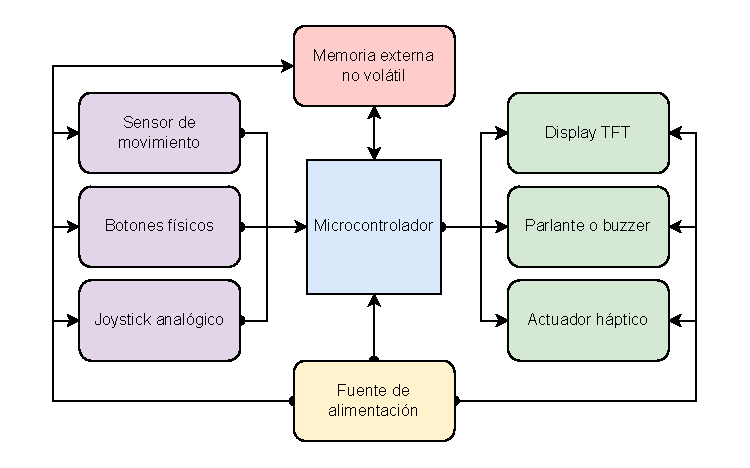
\includegraphics[width=.85\textwidth]{../Figuras/diagrama_bloques_proyecto.pdf}
\caption{Diagrama en bloques del sistema.}
\label{fig:diagBloques}
\end{figure}

\vspace{25px}

%{propuesta de valor}
El presente proyecto no se plantea como un producto de innovación con proyección comercial, pero se distingue por reinterpretar el concepto de consola portátil clásica desde una perspectiva actual. A partir de una arquitectura simple y dedicada, centrada en un único juego, se incorporan características técnicas poco comunes en dispositivos de este tipo, como el uso de un microcontrolador de 32 bits, pantalla a color, sensores de movimiento, retroalimentación háptica y almacenamiento persistente del estado del juego.


\section{2. Identificación y análisis de los interesados}
\label{sec:interesados}


\begin{table}[ht]
%\caption{Identificación de los interesados}
%\label{tab:interesados}
\begin{tabularx}{\linewidth}{@{}|l|L{4.7cm}|X|l|@{}}
\hline
\rowcolor[HTML]{C0C0C0} 
Rol           & Nombre y Apellido & Organización 	& Puesto 	\\ \hline
%Auspiciante   & \authorname     &  FIUBA        	&  -      	\\ \hline
Cliente       & \clientename      &\empclientename	&       	\\ \hline
%Impulsor      &                   &              	&        	\\ \hline
Responsable   & \authorname       & FIUBA        	& Alumno 	\\ \hline
%Colaboradores &                   &              	&        	\\ \hline
Orientador    & \supname	      & \pertesupname 	& Director del Trabajo Final \\ \hline
%Equipo        & miembro1 \newline 
%				miembro2          &              	&        	\\ \hline
%Opositores    &                   &              	&        	\\ \hline
Usuario final &  Entusiastas de sistemas embebidos o videojuegos retro &   	&   	\\ \hline
\end{tabularx}
\end{table}

\begin{itemize}
	\item Cliente: al tratarse de un proyecto académico, se utilizará la figura de cliente a nombre del autor y responsable.
	\item Responsable: será el autor del presente documento, encargado del desarrollo del prototipo y del cumplimiento de los requerimientos pautados en la planificación.
	\item Usuario final: personas con conocimientos técnicos básicos o intermedios, interesados en sistemas embebidos y/o videojuegos retro. 
\end{itemize}
% El Director suele ser uno de los orientadores.


\section{3. Propósito del proyecto}
\label{sec:proposito}

Aplicar de forma integrada los conocimientos adquiridos durante el posgrado en una solución técnica concreta, desarrollada de manera autónoma. Se busca abordar un caso representativo de sistemas embebidos que permita ejercitar competencias clave de la carrera, como la gestión de periféricos, la programación en tiempo real y el diseño modular de software. 


\section{4. Alcance del proyecto}
\label{sec:alcance}

El proyecto incluye:
\begin{itemize}
	\item El diseño y construcción de un prototipo funcional de consola portátil de videojuegos.
	\item El desarrollo de un juego de simulación de vuelo, implementado directamente en el firmware.
	\item La integración de periféricos de entrada:
		\begin{itemize}
		\item Botones físicos.
		\item Joystick analógico.
		\item Sensor de movimiento (acelerómetro y/o giroscopio).
		\end{itemize}
	\item La integración de periféricos de salida:
		\begin{itemize}
		\item Pantalla TFT (a color).
		\item Salida sonora mediante parlante o buzzer.
		\item Motor de vibración para retroalimentación háptica.
		\end{itemize}
	\item El almacenamiento del estado del juego en memoria no volátil.
	\item La documentación técnica requerida para su presentación como trabajo final de especialización.
\end{itemize}
El presente proyecto no incluye:
\begin{itemize}
	\item El diseño y/o la fabricación de una placa de circuito impreso (PCB, por \textit{Printed Circuit Board}).
	\item El desarrollo de un entorno ejecutable separado del juego: el firmware no estará diseñado de forma general para admitir juegos en formatos estándar.
	\item Conectividad externa, comunicación inalámbrica o funcionalidades multijugador.
\end{itemize}


\section{5. Supuestos del proyecto}
\label{sec:supuestos}

Para el desarrollo del presente proyecto se supone que: 

\begin{itemize}
	\item Se dispondrá de los materiales y componentes necesarios para el prototipo funcional.
	\item Las horas estimadas de trabajo serán suficientes para cumplir con los objetivos planteados.
	\item Los conocimientos requeridos para avanzar en las distintas etapas del proyecto se alcanzarán durante el transcurso del posgrado en tiempos compatibles con el desarrollo.
	\item La solución planteada es técnicamente viable dentro del alcance y recursos definidos.
	\item El responsable dispondrá de dedicación a tiempo completo hasta culminar el proyecto.
\end{itemize}


\section{6. Requerimientos}
\label{sec:requerimientos}

Los requerimientos del proyecto son los siguientes:

\begin{enumerate}
	\item Requerimientos de hardware:
	\begin{enumerate}
		\item El prototipo deberá montarse en \textit{protoboard} o soldarse sobre placas de experimentación.
		\item El prototipo deberá alimentarse a través de una batería.
		\item El prototipo deberá integrar un sensor capaz de medir la inclinación en al menos dos ejes.
		\item El prototipo deberá integrar un joystick analógico con capacidad de lectura en dos ejes.
		\item El prototipo deberá incluir botones tipo switch para funciones definidas.
		\item El prototipo deberá incorporar una pantalla capaz de mostrar información visual relevante para el juego.
		\item El prototipo deberá incluir un mecanismo para emitir sonidos o alertas sonoras.
		\item El prototipo deberá integrar un motor de vibración capaz de generar retroalimentación háptica.
		\item El prototipo deberá contar con memoria no volátil para el almacenamiento persistente del estado del juego.
	\end{enumerate}
	\item Requerimientos de firmware:
	\begin{enumerate}
		\item El firmware deberá implementar la lógica para interpretar los datos del sensor de inclinación y el joystick para controlar el modelo de vuelo (cabeceo, alabeo, giro, velocidad).
		\item El firmware deberá incluir un demo de juego integrado que permita demostrar la lógica implementada y la funcionalidad de los periféricos de entrada y salida.
		\item El firmware deberá gestionar la visualización de la información del juego en la pantalla.
		\item El firmware deberá ser capaz de reproducir las alertas sonoras necesarias.
		\item El firmware deberá controlar la activación y duración del motor de vibración en función de los eventos del juego.
		\item El firmware deberá implementar la lógica para guardar y cargar el estado del juego en la memoria no volátil.
		\item El firmware deberá detectar las pulsaciones de los botones y activar las funcionalidades correspondientes (inicio/fin, pausa, guardar, mapa, etc...).
	\end{enumerate}
	\item Requerimientos de documentación:
	\begin{enumerate}
		\item Diagrama de conexión de módulos.
		\item Video demostrativo del uso de las funcionalidades requeridas.
		\item Informe de avance.
		\item Memoria técnica.
	\end{enumerate}
	\item Requerimientos opcionales:
	\begin{enumerate}
		% \item El firmware podrá utilizar un sistema operativo de tiempo real (RTOS por sus siglas en inglés) para gestionar tareas concurrentes como lectura de sensores y salida de señales.
		\item El firmware podrá incluir gráficos a color para representar la interfaz de usuario (UI por sus siglas en inglés).
		\item El sistema podrá incluir uno o varios selectores de niveles para aspectos como: el volumen de las señales audio, el nivel de vibración de la consola, modos de visualización diferentes para debug o gráficos, entre otras opciones posibles.
	\end{enumerate}
\end{enumerate}

\section{7. Historias de usuarios (\textit{Product backlog})}
\label{sec:backlog}

Escalas utilizadas para asignar \textit{story points}:
\begin{enumerate}
	\item Complejidad:
	\begin{itemize}
		\item Baja complejidad: 1 punto
		\item Media complejidad: 3 puntos
		\item Alta complejidad: 5 puntos
	\end{itemize}
	\item Cantidad de trabajo:
	\begin{itemize}
		\item Poco trabajo: 1 punto
		\item Cantidad de trabajo media: 2 puntos
		\item Mucho trabajo: 3 puntos
	\end{itemize}
	\item Incertidumbre asociada:
	\begin{itemize}
		\item  Baja incertidumbre: 2 puntos
		\item  Incertidumbre media: 5 puntos
		\item  Alta incertidumbre: 8 puntos
	\end{itemize}
\end{enumerate}

% \textbf{Épica 1:} Control e interacción del usuario con el demo de juego

	\textbf{HU1: control intuitivo por inclinación.} Como usuario, quiero controlar el cabeceo (\textit{pitch}) y el alabeo (\textit{roll}) de la aeronave inclinando la consola, para tener una experiencia de control más natural e inmersiva.

	% Criterios de aceptación:
	% \begin{itemize}
	% 	\item El sistema interpreta la inclinación de la consola en los ejes X e Y como comandos de alabeo y cabeceo respectivamente.
	% 	\item La respuesta del modelo de vuelo a la inclinación es inmediata y fluida, sin latencia perceptible.
	% 	\item El control debe estar calibrado en un rango usable (sin saturar los extremos).
	% 	\item Se pueden realizar movimientos suaves y precisos con pequeñas inclinaciones.
	% \end{itemize}
	% \textit{Story points}: 13 (complejidad: 3, trabajo: 2, incertidumbre: 5)
	\begin{itemize}
		\item Complejidad media (3 p) porque requiere integrar el sensor de inclinación y procesar sus datos.
		\item Trabajo medio (2 p) porque requiere trabajo de hardware y software. 
		\item Incertidumbre media (5 p) porque requiere evaluar si se requerirán filtros y de qué tipo para el procesamiento de los datos del sensor. 
	\end{itemize}
	\textit{Story points}: 3+2+5=10, redondeo Fibonacci: 13 puntos.

	\textbf{HU2: maniobras precisas con el joystick.} Como usuario, quiero usar el joystick analógico para controlar el giro (\textit{yaw}) y la velocidad de la aeronave, para poder realizar maniobras precisas y ajustar mi trayectoria.

	% Criterios de aceptación:
	% \begin{itemize}
	% 	\item El movimiento horizontal del joystick controla el ángulo de giro de la aeronave de forma proporcional.
	% 	\item El movimiento vertical del joystick controla la velocidad de avance de la aeronave.
	% 	\item El control de giro es suave y permite realizar ajustes finos.
	% \end{itemize}
	% \textit{Story points}: 8 (complejidad: 3, trabajo: 2, incertidumbre: 2)
	\begin{itemize}
		\item Complejidad media (3 p) porque requiere integrar el joystick y mapear sus rangos.
		\item Trabajo medio (2 p) porque requiere trabajo de hardware y software. 
		\item Incertidumbre baja (2 p) porque el módulo de joystick es simple de utilizar. 
	\end{itemize}
	\textit{Story points}: 3+2+2=7, redondeo Fibonacci: 8 puntos.
		
		
	\textbf{HU3: inicio y fin de sesión sencillos.} Como usuario, quiero poder iniciar el juego rápidamente al encender la consola y finalizarla fácilmente cuando termine de jugar para gestionar eficientemente mi tiempo de juego.

	% Criterios de aceptación:
	% \begin{itemize}
	% 	\item Al presionar el botón de ``Inicio", la demostración del juego comienza en un estado predefinido.
	% 	\item Al presionar el botón de ``Finalizar", el juego se detiene y la consola vuelve a un menú principal o estado de espera.
	% \end{itemize}
	% \textit{Story points}: 5 (complejidad: 1, trabajo: 1, incertidumbre: 2)
	\begin{itemize}
		\item Complejidad baja (1 p) porque es una funcionalidad simple una vez que el sistema esta funcionando.
		\item Trabajo bajo (1 p) porque requiere trabajo mayormente de software. 
		\item Incertidumbre baja (2 p) ya que no requiere tomar decisiones específicas para su implementación. 
	\end{itemize}
	\textit{Story points}: 1+1+2=4, redondeo Fibonacci: 5 puntos.
		
% \textbf{Épica 2:} Visualización del entorno y mapa

	\textbf{HU4: información clara del estado.} Como usuario, quiero ver en pantalla información clave como mi velocidad, dirección y posición, para estar siempre informado sobre el estado de mi juego.

	% Criterios de aceptación:
	% \begin{itemize}
	% 	\item La velocidad, dirección y posición actual de la aeronave se representan visualmente en la pantalla.
	% 	\item Los cambios en la velocidad, dirección y posición se reflejan en la pantalla en tiempo real (sin lags perceptibles).
	% \end{itemize}
	% \textit{Story points}: 21 (complejidad: 5, trabajo: 2, incertidumbre: 8)
	\begin{itemize}
		\item Complejidad alta (5 p) porque requiere la configuración apropiada de la pantalla con sus métodos de graficación y la integración de diversas variables de estado del juego.
		\item Trabajo medio (2 p) ya que, una vez definidas las variables y el módulo gráfico, debería ser bastante trivial graficar dichas variables. 
		\item Incertidumbre alta (8 p) porque aún no se encuentra definido el método con el que se renderizarán los gráficos en la pantalla. 
	\end{itemize}
	\textit{Story points}: 5+2+8=15, redondeo Fibonacci: 21 puntos.
		
	\textbf{HU5: visualizar ubicación en el mapa.} Como usuario, quiero ver la posición actual de la aeronave en el mapa, para tener una referencia de navegación.

	% Criterios de aceptación:
	% \begin{itemize}
	% 	\item Al presionar el botón de ``Mapa", se muestra una representación del entorno de vuelo.
	% 	\item La posición actual de la aeronave se indica claramente en el mapa.
	% 	\item El mapa es legible y proporciona una orientación básica del entorno.
	% \end{itemize}
	% \textit{Story points}: 21 (complejidad: 5, trabajo: 3, incertidumbre: 8)
	\begin{itemize}
		\item Complejidad alta (5 p) porque requiere la configuración apropiada de la pantalla con sus métodos de graficación y el diseño de la interfaz del mapa.
		\item Trabajo alto (3 p) ya que requiere graficar elementos varios definidos en el mapa además de la posición de la aeronave. 
		\item Incertidumbre alta (8 p) porque aún no se encuentra definido el método con el que se renderizarán los gráficos en la pantalla ni el diseño de la interfaz gráfica. 
	\end{itemize}
	\textit{Story points}: 5+3+8=16, redondeo Fibonacci: 21 puntos.
		
% \textbf{Épica 3:} Audio y retroalimentación háptica

	\textbf{HU6: sonidos y alertas.} Como usuario, quiero que el sistema emita sonidos o señales acústicas distintivas y relevantes durante el juego, para recibir retroalimentación auditiva.

	% Criterios de aceptación:
	% \begin{itemize}
	% 	\item Se generan al menos dos sonidos distintos para diferentes eventos del juego.
	% 	\item Los sonidos son claramente audibles.
	% 	\item La emisión de sonido está sincronizada con el evento que la provoca.
	% \end{itemize}
	% \textit{Story points}: 8 (complejidad: 3, trabajo: 2, incertidumbre: 2)
	\begin{itemize}
		\item Complejidad media (3 p) porque requiere investigación sobre la implementación del audio.
		\item Trabajo medio (2 p) porque requiere trabajo de hardware y software. 
		\item Incertidumbre baja (2 p) ya que se asume que el módulo seleccionado para audio será simple de utilizar. 
	\end{itemize}
	\textit{Story points}: 3+2+2=7, redondeo Fibonacci: 8 puntos.
		
	\textbf{HU7: generar vibración durante el juego.} Como usuario, quiero que el dispositivo genere vibración en ciertos eventos del juego, para tener una experiencia más inmersiva y física.

	% Criterios de aceptación:
	% \begin{itemize}
	% 	\item El motor de vibración se activa ante al menos un evento definido.
	% 	\item La duración de la vibración es perceptible y coherente con el evento.
	% \end{itemize}
	% \textit{Story points}: 8 (complejidad: 1, trabajo: 2, incertidumbre: 5)
	\begin{itemize}
		\item Complejidad baja (1 p) ya que se utilizará un módulo de driver que debería resolver la mayor complejidad de la implementación.
		\item Trabajo medio (2 p) porque requiere trabajo de hardware y software. 
		\item Incertidumbre media (5 p) porque aún no se encuentran definidos los eventos que generarán las vibraciones y porque la implementación involucra un módulo que no se utilizó anteriormente. 
	\end{itemize}
	\textit{Story points}: 1+2+5=8, redondeo Fibonacci: 8 puntos.
		
% \textbf{Épica 4:} Gestión del estado del juego

	\textbf{HU8: guardar el estado actual de la partida.} Como usuario, quiero poder guardar el estado del juego en curso, para retomar el progreso más adelante.

	% Criterios de aceptación:
	% \begin{itemize}
	% 	\item El sistema almacena las variables clave del estado del juego en memoria no volátil.
	% 	\item Se proporciona una señal de confirmación visual y/o sonora al guardar.
	% 	\item El estado guardado se puede cargar al reiniciar el entorno.
	% \end{itemize}
	% \textit{Story points}: 13 (complejidad: 3, trabajo: 3, incertidumbre: 5)
	\begin{itemize}
		\item Complejidad media (3 p) porque requiere almacenar la totalidad de la información necesaria para definir el estado de la partida.
		\item Trabajo alto (3 p) porque requiere bastante trabajo de hardware y software. 
		\item Incertidumbre media (5 p) ya que aún no se han definido las variables a preservar ni el formato de almacenamiento. 
	\end{itemize}
	\textit{Story points}: 3+3+5=11, redondeo Fibonacci: 13 puntos.
		
	\textbf{HU9: elegir cómo empezar.} Como usuario, quiero poder seleccionar entre continuar una partida previamente guardada o descartarla e iniciar una nueva, para tener control sobre cómo empezar cada sesión de juego.

	% Criterios de aceptación:
	% \begin{itemize}
	% 	\item Si existe un estado guardado, el sistema ofrece la opción de continuar o iniciar una nueva partida.
	% 	\item Si no hay estado guardado, el juego comienza automáticamente.
	% 	\item Se indica claramente la opción seleccionada por el usuario.
	% \end{itemize}
	% \textit{Story points}: 5 (complejidad: 1, trabajo: 2, incertidumbre: 2)
	\begin{itemize}
		\item Complejidad baja (1 p) ya que la mayor complejidad será abordada al definir cómo guardar y recuperar el estado.
		\item Trabajo medio (2 p) porque requiere trabajo de hardware y software. 
		\item Incertidumbre baja (2 p) porque solo resta definir cómo se realizará el descarte de la partida anterior. 
	\end{itemize}
	\textit{Story points}: 1+2+2=5, redondeo Fibonacci: 5 puntos.

	\textbf{HU10: pausar y retomar el juego.} Como usuario, quiero poder pausar la partida en cualquier momento para tomar un descanso y luego reanudarla exactamente donde la dejé.

	% Criterios de aceptación:
	% \begin{itemize}
	% 	\item Al presionar el botón de ``Pausa" por primera vez, el juego se detiene.
	% 	\item Al presionar el botón de ``Pausa" nuevamente, el juego se restablece en el mismo estado que estaba antes de pausar.
	% 	\item Se indica claramente en pantalla cuando el juego está pausado.
	% \end{itemize}
	% \textit{Story points}: 5 (complejidad: 1, trabajo: 2, incertidumbre: 2)
	\begin{itemize}
		\item Complejidad baja (1 p) ya que solo debería implicar un periodo en el que no se actualice el estado del juego.
		\item Trabajo medio (2 p) porque implica actualizar en pantalla un mensaje que indique las acciones de pausado y reanudación de la partida. 
		\item Incertidumbre baja (2 p) ya que solo resta definir la forma en la que se comunicará el estado pausado al usuario. 
	\end{itemize}
	\textit{Story points}: 1+2+2=5, redondeo Fibonacci: 5 puntos.
		
% \textbf{Épica 5:} Documentación del proyecto

	\textbf{HU11: entender las conexiones del hardware.} Como cliente, quiero disponer de un diagrama de conexión de los módulos para comprender la arquitectura física del prototipo.

	% Criterios de aceptación:
	% \begin{itemize}
	% 	\item El diagrama muestra todos los módulos de hardware principales.
	% 	\item Las conexiones entre los módulos son claras y fáciles de seguir.
	% 	\item Se incluyen etiquetas descriptivas para cada componente y conexión.
	% \end{itemize}
	% \textit{Story points}: 5 (complejidad: 1, trabajo: 1, incertidumbre: 2)
	\begin{itemize}
		\item Complejidad baja (1 p).
		\item Trabajo bajo (1 p). 
		\item Incertidumbre baja (2 p). 
	\end{itemize}
	\textit{Story points}: 1+1+2=4, redondeo Fibonacci: 5 puntos.
		
	\textbf{HU12: ver el prototipo en acción.} Como cliente, quiero ver un video que muestre las funcionalidades del prototipo para comprobar el cumplimiento de lo solicitado.

	% Criterios de aceptación:
	% \begin{itemize}
	% 	\item El video demuestra las funcionalidades clave de las historias de usuario implementadas.
	% 	\item El video es claro, bien enfocado y con una duración adecuada.
	% 	\item Se pueden observar los criterios de aceptación de las funcionalidades en el video.
	% \end{itemize}
	% \textit{Story points}: 5 (complejidad: 1, trabajo: 2, incertidumbre: 2)
	\begin{itemize}
		\item Complejidad baja (1 p).
		\item Trabajo medio (2 p). 
		\item Incertidumbre baja (2 p). 
	\end{itemize}
	\textit{Story points}: 1+2+2=5, redondeo Fibonacci: 5 puntos.
		
	\textbf{HU13: seguir el proceso de desarrollo.} Como cliente, quiero recibir al menos un informe de avance para entender la evolución del proyecto.

	% Criterios de aceptación:
	% \begin{itemize}
	% 	\item Se entrega al menos un informe de avance.
	% 	\item El informe documentan los avances realizados y los cambios respecto al plan (si se presentan).
	% 	\item El informe es claro y proporciona una visión del progreso del proyecto.
	% \end{itemize}
	% \textit{Story points}: 8 (complejidad: 3, trabajo: 2, incertidumbre: 2)
	\begin{itemize}
		\item Complejidad media (3 p).
		\item Trabajo medio (2 p). 
		\item Incertidumbre baja (2 p). 
	\end{itemize}
	\textit{Story points}: 3+2+2=7, redondeo Fibonacci: 8 puntos.
		
	\textbf{HU14: comprender las decisiones técnicas.} Como cliente, quiero tener acceso a una memoria técnica para entender en detalle el diseño y la implementación del prototipo.

	% Criterios de aceptación:
	% \begin{itemize}
	% 	\item La memoria técnica describe la arquitectura del hardware y del software.
	% 	\item Se explican las decisiones de diseño clave y sus justificaciones.
	% 	\item La documentación es clara, organizada y proporciona suficiente detalle técnico.
	% \end{itemize}
	% \textit{Story points}: 13 (complejidad: 3, trabajo: 3, incertidumbre: 5)
	\begin{itemize}
		\item Complejidad media (3 p).
		\item Trabajo alto (3 p). 
		\item Incertidumbre media (5 p). 
	\end{itemize}
	\textit{Story points}: 3+3+5=11, redondeo Fibonacci: 13 puntos.


\section{8. Entregables principales del proyecto}
\label{sec:entregables}

% \begin{consigna}{red}
Los entregables del proyecto son:

\begin{itemize}
	\item Plan de trabajo.
	\item Memoria del proyecto. 
	\item Prototipo funcional. 
	\item Diagrama de conexiones.
	\item Código fuente.
\end{itemize}
% \end{consigna}

\section{9. Desglose del trabajo en tareas}
\label{sec:wbs}

\begin{enumerate}	
	\item	Desarrollo del hardware. (34 h)
	\begin{enumerate}	
	\item	Selección y adquisición de componentes. (4 h)
	\begin{enumerate}	
	\item	Confirmación de los componentes existentes y verificación de su idoneidad. (2 h)
	\item	Adquisición de componentes faltantes o adicionales. (2 h)
	\end{enumerate}	
	\item	Montaje del prototipo en \textit{protoboard}. (12 h)
	\begin{enumerate}	
	\item	Planificación del diseño de montaje. (3 h)
	\item	Montaje y cableado del microcontrolador y la fuente de alimentación. (3 h)
	\item	Montaje y cableado del sensor de inclinación. (1 h)
	\item	Montaje y cableado del joystick analógico. (0,5 h)
	\item	Montaje y cableado de los botones. (0,5 h)
	\item	Montaje y cableado de la pantalla. (1 h)
	\item	Montaje y cableado del sistema de audio. (1,5 h)
	\item	Montaje y cableado del motor de vibración. (1,5 h)
	\end{enumerate}	
	\item	Pruebas por componente en \textit{protoboard}. (18 h)
	\begin{enumerate}	
	\item	Prueba de conexión del sensor de inclinación. (5 h)
	\item	Prueba de conexión del joystick analógico. (1 h)
	\item	Prueba de conexión de los botones. (1 h)
	\item	Prueba de conexión de la pantalla. (6 h)
	\item	Prueba de conexión del sistema de audio. (2 h)
	\item	Prueba de conexión del motor de vibración. (3 h)
	\end{enumerate}	
	\end{enumerate}	
	\item	Desarrollo del firmware. (436 h)
	\begin{enumerate}	
	\item	Configuración Inicial del entorno de desarrollo. (1 h)
	\begin{enumerate}	
	\item	Configuración de la placa, pines y periféricos. (1 h)
	\end{enumerate}	
	\item	Implementación de la lógica del sistema. (117 h)
	\begin{enumerate}	
	\item	Desarrollo del módulo de adquisición de señales de entrada. (30 h)
	\item	Desarrollo del módulo de generación de señales de salida. (37 h)
	\begin{enumerate}	
	\item	Módulo de salida: sub-módulo de audio. (4 h)
	\item	Módulo de salida: sub-módulo de vibraciones. (8 h)
	\item	Módulo de salida: sub-módulo de gráficos. (25 h)
	\end{enumerate}	
	\item	Investigación sobre distintos sistemas operativos de tiempo real (RTOS por sus siglas en inglés). (5 h)
	\item	Implementación del RTOS seleccionado. (20 h)
	\item	Diseño e implementación de una máquina de estados para el control general del sistema. (25 h)
	\end{enumerate}	
	\item	Implementación del demo de juego. (55 h)
	\begin{enumerate}	
	\item	Diseño de la lógica del demo de juego. (25h)
	\item	Desarrollo de la máquina de estados del juego. (10 h)
	\item	Integración de la lógica de control con el demo de juego y la máquina de estados del juego. (20 h)
	\end{enumerate}	
	\item	Detección de entradas simples. (11 h)
	\begin{enumerate}	
	\item	Implementación de la detección de pulsaciones de los botones. (3 h)
	\item	Implementación de la lectura de los datos del joystick analógico. (3 h)
	\item	Integración de las entradas de botones y joystick con la máquina de estados del sistema. (5 h)
	\end{enumerate}	
	\item	Detección de inclinación. (18 h)
	\begin{enumerate}	
	\item	Implementación de la lectura de los datos del sensor de inclinación. (5 h)
	\item	Procesamiento de los datos del acelerómetro para obtener la inclinación. (3 h)
	\item	Integración de la detección de inclinación con la lógica del sistema. (10 h)
	\end{enumerate}	
	\item	Gestión de la interfaz de usuario. (140 h)
	\begin{enumerate}	
	\item	Investigación y aprendizaje de conceptos básicos de graficación en la pantalla. (25 h)
	\item	Inicialización y configuración de la pantalla para la visualización. (20 h)
	\item	Implementación de la visualización del estado de la aeronave. (40 h)
	\item	Implementación de la visualización del mapa y la posición. (35 h)
	\item	Implementación de la lógica para mostrar/ocultar elementos de la UI. (20 h)
	\end{enumerate}	
	\item	Implementación de la reproducción de audio. (18 h)
	\begin{enumerate}	
	\item	Investigación sobre modos de generación y/o reproducción de audio en sistemas embebidos. (5 h)
	\item	Implementación de la capacidad de reproducir audio. (8 h)
	\item	Lógica para activar los sonidos en eventos específicos del juego. (5 h)
	\end{enumerate}	
	\item	Implementación del control de vibración. (33 h)
	\begin{enumerate}	
	\item	Investigación sobre generación de vibración con distintos patrones. (8 h)
	\item	Implementación de la capacidad de controlar el motor de vibración. (15 h)
	\item	Lógica para activar la vibración en eventos específicos del juego. (10 h)
	\end{enumerate}	
	\item	Gestión del estado del juego. (43 h)
	\begin{enumerate}	
	\item	Definición de las variables del estado del juego a persistir. (8 h)
	\item	Implementación de la lógica para guardar el estado del juego en memoria no volátil. (15 h)
	\item	Implementación de la lógica para cargar el estado del juego desde memoria no volátil. (15 h)
	\item	Implementación de la lógica para pausar y reanudar el juego. (5 h)
	\end{enumerate}	
	\item	Integración del demo de juego. (Tarea continua)
	\end{enumerate}	
	\item	Pruebas y verificación. (55 h)
	\begin{enumerate}	
	\item	Pruebas de control por inclinación. (8 h)
	\item	Pruebas de control por joystick. (5 h)
	\item	Pruebas de inicio y Fin de sesión. (8 h)
	\item	Pruebas de visualización del estado de la aeronave. (8 h)
	\item	Pruebas de visualización del mapa. (8 h)
	\item	Pruebas de audio. (3 h)
	\item	Pruebas de vibración. (5 h)
	\item	Pruebas de guardado y carga del estado. (5 h)
	\item	Pruebas de pausa y reanudación. (5 h)
	\item	Pruebas de integración. (Tarea continua)
	\end{enumerate}	
	\item	Documentación. (115 h)
	\begin{enumerate}	
	\item	Creación del diagrama de conexión de módulos. (15 h)
	\item	Grabación y edición del video demostrativo. (20 h)
	\item	Elaboración del informe de avance. (30 h)
	\item	Elaboración de la memoria técnica. (50 h)
	\end{enumerate}	
		
	\item	Tareas opcionales (se abordarán solo si el tiempo y los recursos lo permiten). (141 h)
	\begin{enumerate}	
	\item	Implementación de gráficos a color. (78 h)
	\begin{enumerate}	
	\item	Investigación de la capacidad de la pantalla. (9 h)
	\item	Diseño de gráficos y paleta de colores. (20 h)
	\item	Modificación de las rutinas de dibujo. (20 h)
	\item	Actualización de los elementos visuales. (20 h)
	\item	Pruebas de la visualización a color. (9 h)
	\end{enumerate}	
	\item	Implementación de selectores (por selector). (28 h)
	\begin{enumerate}	
	\item	Diseño de la interfaz del selector. (5 h)
	\item	Implementación de la lógica de navegación del selector. (10 h)
	\item	Implementación de la lógica de aplicación del valor seleccionado. (8 h)
	\item	Pruebas del selector y su correcta funcionalidad. (5 h)
	\end{enumerate}	
	\item	Montaje en placas de experimentación. (35 h)
	\begin{enumerate}	
	\item	Diseño del layout para placas de experimentación. (10 h)
	\item	Soldadura de los componentes en las placas de experimentación. (15 h)
	\item	Pruebas de alimentación de los componentes. (2 h)
	\item	Pruebas de continuidad y cortocircuitos. (3 h)
	\item	Pruebas de funcionamiento de cada componente. (5 h)
	\end{enumerate}	
	\end{enumerate}	
	\end{enumerate}	
	Cantidad total de horas (sin contemplar opcionales): 640.	
		
	Cantidad de horas de ingeniería (sin contemplar opcionales ni documentación): 525.	

\section{10. Diagrama de Activity On Node}
\label{sec:AoN}

\begin{figure}[htpb]
\centering 
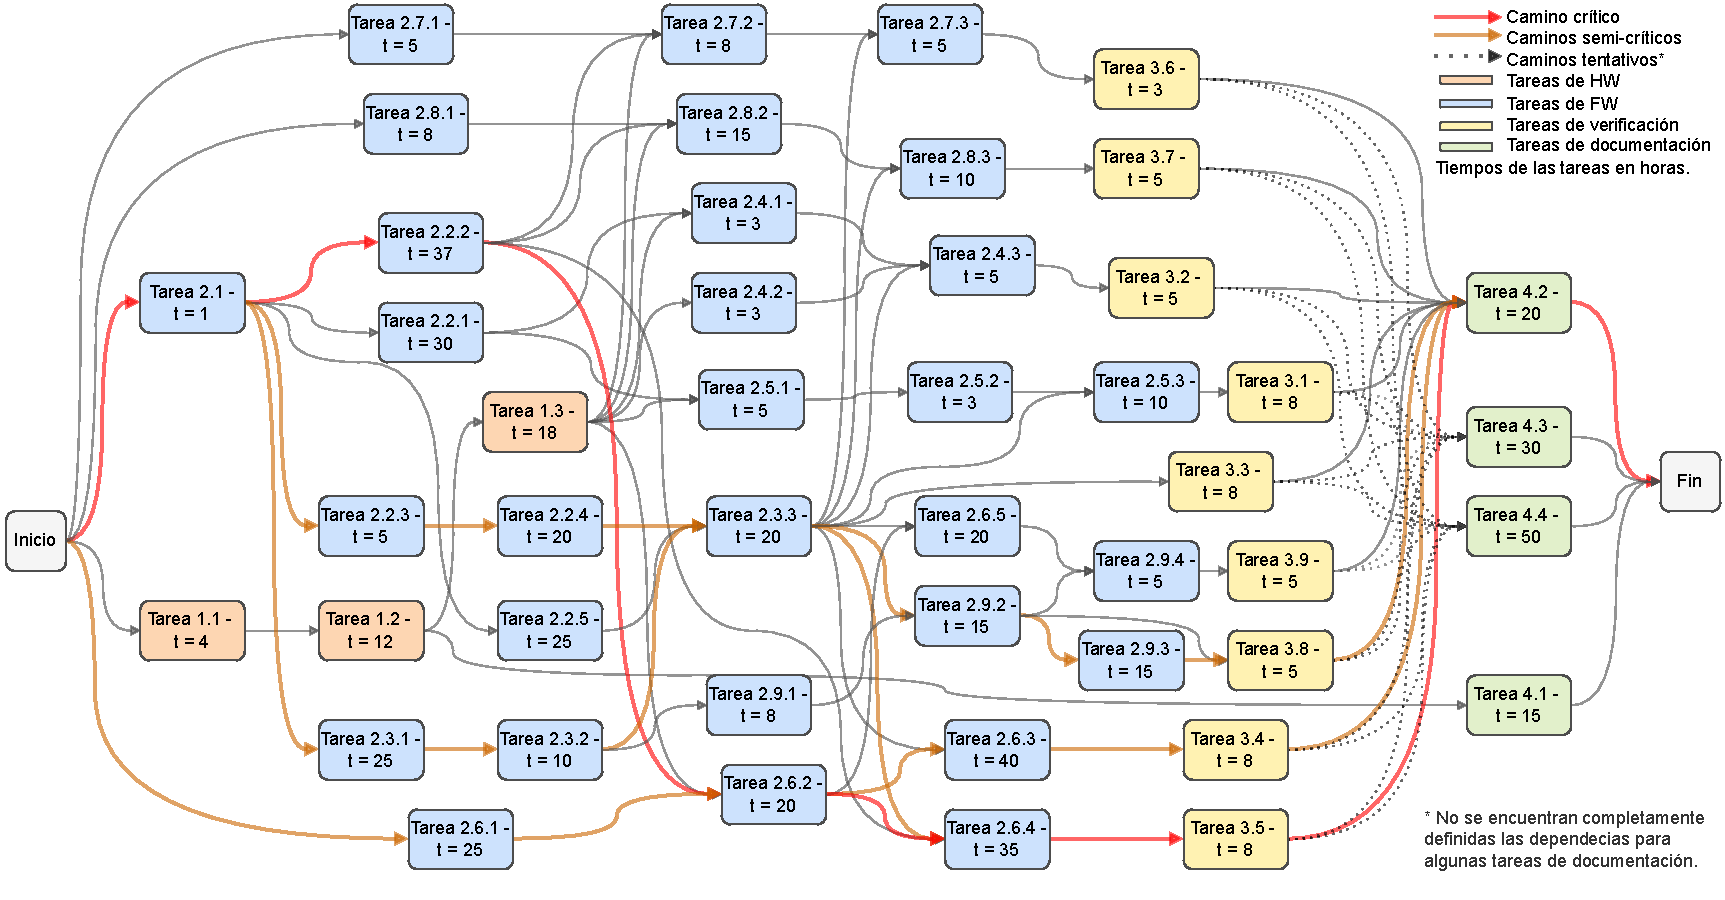
\includegraphics[width=\textwidth]{../Figuras/aon.drawio.pdf}
\caption{Diagrama de \textit{Activity on Node}.}
\label{fig:AoN}
\end{figure}

Camino Crítico: 
\begin{itemize}
	\item Inicio \textrightarrow  Tarea 2.1 \textrightarrow  Tarea 2.2.2 \textrightarrow  Tarea 2.6.2 \textrightarrow  Tarea 2.6.4 \textrightarrow  Tarea 3.5 \textrightarrow  Tarea 4.2 \textrightarrow  Fin (121 h)
\end{itemize}

Caminos semi críticos:
\begin{itemize}
	\item Inicio \textrightarrow  Tarea 2.6.1 \textrightarrow  Tarea 2.6.2 \textrightarrow  Tarea 2.6.3 \textrightarrow  Tarea 3.4 \textrightarrow  Tarea 4.2 \textrightarrow  Fin (113 h)
	\item Inicio \textrightarrow  Tarea 2.1 \textrightarrow  Tarea 2.3.1 \textrightarrow  Tarea 2.3.2 \textrightarrow  Tarea 2.3.3 \textrightarrow  Tarea 2.9.2 \textrightarrow  Tarea 2.9.3 \textrightarrow  3.8 \textrightarrow  Tarea 4.2 \textrightarrow  Fin (111 h)
	\item Inicio \textrightarrow  Tarea 2.1 \textrightarrow  Tarea 2.2.3 \textrightarrow  Tarea 2.2.4 \textrightarrow  Tarea 2.3.3 \textrightarrow  Tarea 2.6.4 \textrightarrow  Tarea 3.5 \textrightarrow  4.2 \textrightarrow  Fin (109 h)
	\item Inicio \textrightarrow  Tarea 2.6.1 \textrightarrow  Tarea 2.6.2 \textrightarrow  2.6.4 \textrightarrow  Tarea 3.5 \textrightarrow  Tarea 4.2 \textrightarrow  Fin (108 h)
\end{itemize}


\section{11. Diagrama de Gantt}
\label{sec:gantt}

En la figura \ref{fig:gantt_proyecto1} se puede observar el diagrama de Gantt del proyecto. Se presentan las tareas de ingeniería hasta el segundo nivel de jerarquía de la estructura de desglose de trabajo (EDT) y las tareas de verificación y documentación hasta el primer nivel de jerarquía, a modo de facilitar la legibilidad del diagrama. 

Para el cálculo de las fechas de inicio y fin se consideraron tanto las dependencias entre tareas como las restricciones de recursos necesarios. La restricción más relevante es la de recursos humanos, ya que se cuenta con un único responsable y desarrollador. Se estimó una carga de trabajo de 6 horas diarias durante 5 días a la semana. El detalle de las fechas, duración y descripción de las tareas puede observarse en el cuadro \ref{tab:gantt}.

% Define custom colors for groups
\definecolor{hardwarecolor}{HTML}{FFE6CC} % Light orange for Hardware
\definecolor{firmwarecolor}{HTML}{DAE8FC} % Light blue for Firmware
\definecolor{verificationcolor}{HTML}{FFF2CC} % Light yellow for Verification
\definecolor{documentationcolor}{HTML}{D5E8D4} % Light green for Documentation 

\makeatletter
\def\pgfcalendarmonthshortername#1{%
  \pgfutil@translate{\ifcase#1\or Ene\or Feb\or Mar\or Abr\or
    May\or Jun\or Jul\or Ago\or Sep\or Oct\or
    Nov\or Dic\fi}%
}
% \begin{landscape}
\begin{figure}[htpb]
    \begin{center}
      \begin{ganttchart}[
        % vgrid={*{1}{draw=gray!50, dashed}},
  		% hgrid,
%  		time slot unit=day,
  		time slot format=isodate,
		calendar week text = {W\currentweek{}},
        x unit=0.075cm,
		y unit title=0.7cm,
		y unit chart=0.6cm,
		bar height=0.5,
		group height=0.6,
		% milestone/.append style={xscale=4}
		milestone left shift =-1,
    	milestone right shift =2
      ]{2025-06-16}{2025-11-20}  % Start and End dates for the entire chart

	  \gantttitlecalendar{year, month=shortername} \\

		% Hardware Group
        \ganttgroup[group/.append style={fill=hardwarecolor}]{1. Hardware}{2025-06-16}{2025-06-24} \\
		\ganttbar[bar/.append style={fill=hardwarecolor}]{Tarea 1.1}{2025-06-16}{2025-06-17} \\
		\ganttbar[bar/.append style={fill=hardwarecolor}]{Tarea 1.2}{2025-06-17}{2025-06-19} \\
		\ganttbar[bar/.append style={fill=hardwarecolor}]{Tarea 1.3}{2025-06-19}{2025-06-24} \\

		% Firmware Group
		\ganttgroup[group/.append style={fill=firmwarecolor}]{2. Firmware}{2025-06-24}{2025-10-09} \\
		\ganttbar[bar/.append style={fill=firmwarecolor}]{Tarea 2.1}{2025-06-24}{2025-06-25} \\
		\ganttbar[bar/.append style={fill=firmwarecolor}]{Tarea 2.2}{2025-06-25}{2025-07-23} \\
		\ganttbar[bar/.append style={fill=firmwarecolor}]{Tarea 2.3}{2025-07-23}{2025-08-06} \\
		\ganttbar[bar/.append style={fill=firmwarecolor}]{Tarea 2.4}{2025-08-06}{2025-08-08} \\
		\ganttbar[bar/.append style={fill=firmwarecolor}]{Tarea 2.5}{2025-08-08}{2025-08-13} \\
		\ganttbar[bar/.append style={fill=firmwarecolor}]{Tarea 2.6}{2025-08-13}{2025-09-16} \\
		\ganttbar[bar/.append style={fill=firmwarecolor}]{Tarea 2.7}{2025-09-16}{2025-09-19} \\
		\ganttbar[bar/.append style={fill=firmwarecolor}]{Tarea 2.8}{2025-09-19}{2025-09-29} \\
		\ganttbar[bar/.append style={fill=firmwarecolor}]{Tarea 2.9}{2025-09-29}{2025-10-09} \\

		% Verificación Group
		\ganttgroup[group/.append style={fill=verificationcolor}]{3. Verificación}{2025-10-09}{2025-10-23} \\
		% Documentación Group
		\ganttgroup[group/.append style={fill=documentationcolor}]{4. Documentación}{2025-10-23}{2025-11-20}  \\

	\end{ganttchart}
\end{center}
\caption{Diagrama de Gantt del proyecto.}
\label{fig:gantt_proyecto1}
\end{figure}


\begin{table}[ht]
	\begin{tabularx}{\linewidth}{@{}|C{1.5cm}|X|c|c|c|@{}}
	\hline
	\rowcolor[HTML]{C0C0C0} 
        Número de tarea & Descripción & Duración & Fecha inicio & Fecha finalización \\ \hline
		1 & Desarrollo del hardware & 34 h & 16/06/2025 & 24/06/2025 \\ \hline
        1.1 & Selección y adquisición de componentes & 4 h & 16/06/2025 & 17/06/2025 \\ \hline
        1.2 & Montaje del prototipo en \textit{protoboard} & 12 h & 17/06/2025 & 19/06/2025 \\ \hline
        1.3 & Pruebas por componente en \textit{protoboard} & 18 h & 19/06/2025 & 24/06/2025 \\ \hline
		2 & Desarrollo del firmware & 436 h & 24/06/2025 & 09/10/2025 \\ \hline
        2.1 & Configuración inicial del entorno de desarrollo & 1 h & 24/06/2025 & 25/06/2025 \\ \hline
        2.2 & Implementación de la lógica del sistema & 117 h & 25/06/2025 & 23/07/2025 \\ \hline
        2.3 & Implementación del demo de juego & 55 h & 23/07/2025 & 06/08/2025 \\ \hline
        2.4 & Detección de entradas simples & 11 h & 06/08/2025 & 08/08/2025 \\ \hline
        2.5 & Detección de inclinación & 18 h & 08/08/2025 & 13/08/2025 \\ \hline
        2.6 & Gestión de la interfaz de usuario & 140 h & 13/08/2025 & 16/09/2025 \\ \hline
        2.7 & Implementación de la reproducción de audio & 18 h & 16/09/2025 & 19/09/2025 \\ \hline
        2.8 & Implementación del control de vibración & 33 h & 19/09/2025 & 29/09/2025 \\ \hline
        2.9 & Gestión del estado del juego & 43 h & 29/09/2025 & 09/10/2025 \\ \hline
        3 & Pruebas y verificación & 55 h & 09/10/2025 & 23/10/2025 \\ \hline
        4 & Documentación & 115 h & 23/10/2025 & 20/11/2025 \\ \hline
    \end{tabularx}
	\caption{Detalle de las tareas para el diagrama de Gantt del proyecto.}
	\label{tab:gantt}
\end{table}

% \end{landscape} 



\section{12. Presupuesto detallado del proyecto}
\label{sec:presupuesto}

En el cuadro \ref{tab:presupuesto} se listan todos los costos asociados al proyecto, expresados en euros (EUR). La cotización de otras monedas de interés al 1 de mayo de 2025 fue la siguiente:

\begin{itemize}
	\item EUR 1 = dólares americanos (USD) 1,1343, presupuesto en USD: 14.843,45. 
	\item EUR 1 = pesos argentinos (ARS) 1328,36, presupuesto en ARG: 17.382.918,96.
\end{itemize}


\begin{table}[ht]
\centering
\begin{tabularx}{\linewidth}{@{}|X|c|r|r|@{}}
\hline
\rowcolor[HTML]{C0C0C0} 
\multicolumn{4}{|c|}{\cellcolor[HTML]{C0C0C0}COSTOS DIRECTOS} \\ \hline
\rowcolor[HTML]{C0C0C0} 
Descripción &
  \multicolumn{1}{c|}{\cellcolor[HTML]{C0C0C0}Cantidad} &
  \multicolumn{1}{c|}{\cellcolor[HTML]{C0C0C0}Valor unitario} &
  \multicolumn{1}{c|}{\cellcolor[HTML]{C0C0C0}Valor total} \\ \hline
Placa STM NUCLEO-F446RE &
  \multicolumn{1}{c|}{1} &
  \multicolumn{1}{c|}{€ 33.99} &
  \multicolumn{1}{c|}{€ 33.99} \\ \hline
Pantalla TFT &
  \multicolumn{1}{c|}{1} &
  \multicolumn{1}{c|}{€ 7.49} &
  \multicolumn{1}{c|}{€ 7.49} \\ \hline
Controlador háptico DRV2605L &
  \multicolumn{1}{c|}{1} &
  \multicolumn{1}{c|}{€ 9,99} &
  \multicolumn{1}{c|}{€ 9,99} \\ \hline
Motor vibración 3V 44000rpm &
  \multicolumn{1}{c|}{5} &
  \multicolumn{1}{c|}{€ 1,44} &
  \multicolumn{1}{c|}{€ 7,21} \\ \hline
Speaker 8 ohm 1W  &
  \multicolumn{1}{c|}{2} &
  \multicolumn{1}{c|}{€ 3,18} &
  \multicolumn{1}{c|}{€ 6,35} \\ \hline
Amplificadores para audio &
  \multicolumn{1}{c|}{5} &
  \multicolumn{1}{c|}{€ 0,27} &
  \multicolumn{1}{c|}{€ 1,33} \\ \hline
Módulo power supply (9V → 5V/3.3V) &
  \multicolumn{1}{c|}{1} &
  \multicolumn{1}{c|}{€ 2,00} &
  \multicolumn{1}{c|}{€ 2,00} \\ \hline
Protoboard &
  \multicolumn{1}{c|}{3} &
  \multicolumn{1}{c|}{€ 2,83} &
  \multicolumn{1}{c|}{€ 8,49} \\ \hline
Cables de conexión (pack) &
  \multicolumn{1}{c|}{1} &
  \multicolumn{1}{c|}{€ 8,59} &
  \multicolumn{1}{c|}{€ 8,59} \\ \hline
Joystick analógico &
  \multicolumn{1}{c|}{1} &
  \multicolumn{1}{c|}{€ 2,00} &
  \multicolumn{1}{c|}{€ 2,00} \\ \hline
Botones tipo switch &
  \multicolumn{1}{c|}{5} &
  \multicolumn{1}{c|}{€ 0,30} &
  \multicolumn{1}{c|}{€ 1,50} \\ \hline
Analizador lógico de 8 canales &
  \multicolumn{1}{c|}{1} &
  \multicolumn{1}{c|}{€ 13,99} &
  \multicolumn{1}{c|}{€ 13,99} \\ \hline
EEPROM SPI 256K (25LC256) &
  \multicolumn{1}{c|}{1} &
  \multicolumn{1}{c|}{€ 1,70} &
  \multicolumn{1}{c|}{€ 1,70} \\ \hline
Acelerómetro GY-521 &
  \multicolumn{1}{c|}{1} &
  \multicolumn{1}{c|}{€ 2,99} &
  \multicolumn{1}{c|}{€ 2,99} \\ \hline
Honorarios profesionales &
  \multicolumn{1}{c|}{640} &
  \multicolumn{1}{c|}{€ 20,00} &
  \multicolumn{1}{c|}{€ 12.800,00} \\ \hline

\multicolumn{3}{|c|}{SUBTOTAL} &
	\multicolumn{1}{c|}{€ 12.906,80} \\ \hline
\rowcolor[HTML]{C0C0C0} 
\multicolumn{4}{|c|}{\cellcolor[HTML]{C0C0C0}COSTOS INDIRECTOS} \\ \hline
\rowcolor[HTML]{C0C0C0} 
Descripción &
  \multicolumn{1}{c|}{\cellcolor[HTML]{C0C0C0}Cantidad} &
  \multicolumn{1}{c|}{\cellcolor[HTML]{C0C0C0}Valor unitario} &
  \multicolumn{1}{c|}{\cellcolor[HTML]{C0C0C0}Valor total} \\ \hline
Servicios de electricidad e internet &
  \multicolumn{1}{c|}{640} &
  \multicolumn{1}{c|}{€ 0,28} &
  \multicolumn{1}{c|}{€ 179,20} \\ \hline
\multicolumn{3}{|c|}{SUBTOTAL} &
	\multicolumn{1}{c|}{€ 179,20} \\ \hline
\rowcolor[HTML]{C0C0C0}
\multicolumn{3}{|c|}{TOTAL} &
   € 13.086,00\\ \hline
\end{tabularx}
\caption{Presupuesto del proyecto.}
	\label{tab:presupuesto}
\end{table}


\section{13. Gestión de riesgos}
\label{sec:riesgos}

% \begin{consigna}{red}
% a) Identificación de los riesgos (al menos cinco) y estimación de sus consecuencias:

En la presente sección se listan los riesgos detectados para el proyecto. Para estimar la severidad y la probabilidad de ocurrencia de cada riesgo se utilizó una escala de 1 a 10, donde 1 corresponde a la menor severidad/ocurrencia y 10 a la mayor.

Riesgo 1. Que las horas estimadas de trabajo no sean suficientes para cumplir con los objetivos planteados.
\begin{itemize}
	\item Severidad (S): 7. Se retrasaría la fecha de presentación del proyecto y su defensa pública.
	\item Ocurrencia (O): 6. No se tiene experiencia en muchos de los aspectos técnicos a trabajar durante el proyecto, por lo que la incertidumbre asociada a la planificación de las horas de trabajo es grande.
\end{itemize}   

Riesgo 2. Que el responsable no pueda dedicar su tiempo completo al proyecto.
\begin{itemize}
	\item Severidad (S): 7. Se retrasaría la fecha de presentación del proyecto y su defensa pública.
	\item Ocurrencia (O): 3. El responsable no asumirá otros compromisos de largo plazo durante el transcurso del proyecto, pero eventos fuera de su control podrían requerir de su atención de todas maneras.
\end{itemize}

Riesgo 3. Que la solución planteada no sea técnicamente viable.
\begin{itemize}
	\item Severidad (S): 9. Se debería cambiar de proyecto.
	\item Ocurrencia (O): 3. Existen dispositivos con elementos de hardware y software similares en el mercado, por lo que no es tan probable que no pueda desarrollarse el proyecto planteado.
\end{itemize}

Riesgo 4. Que los conocimientos del posgrado requeridos para avanzar en las distintas etapas del proyecto no se alcanzaran en tiempos compatibles con el desarrollo.
\begin{itemize}
	\item Severidad (S): 8. Podría ser necesario el retrabajo sobre algún aspecto del proyecto, retrasando la fecha de presentación y su defensa pública.
	\item Ocurrencia (O): 4. El orden de las materias en el posgrado parece ser coherente con la progresión del trabajo necesario para el proyecto.
\end{itemize}

Riesgo 5. Que no se disponga de los materiales y componentes necesarios para el prototipo funcional.
\begin{itemize}
	\item Severidad (S): 8. Podría ser necesario el rediseño de algún aspecto del proyecto y/o la búsqueda de componentes de reemplazo, retrasando la fecha de presentación y su defensa pública.
	\item Ocurrencia (O): 7. El mercado local de componentes electrónicos es escaso y la importación de componentes desde afuera del país suele ser bastante compleja.
\end{itemize}

Riesgo 6. Que la complejidad de graficar en la pantalla el tipo de información requerida sea mayor que la prevista en esta planificación.
\begin{itemize}
	\item Severidad (S): 7. Se retrasaría la fecha de presentación del proyecto y su defensa pública.
	\item Ocurrencia (O): 7. Se desconocen por completo las técnicas de renderizado de imágenes para videojuegos.
\end{itemize}


Estos riesgos se ponderan de acuerdo a la siguiente fórmula:
% \begin{equation}
\[RP N = S * O\]
% \end{equation}
% b) Tabla de gestión de riesgos:      (El RPN se calcula como RPN=SxO)

\begin{table}[htpb]
\centering
\begin{tabularx}{\linewidth}{@{}|X|c|c|c|c|c|c|@{}}
\hline
\rowcolor[HTML]{C0C0C0} 
Riesgo & S & O & RPN & S* & O* & RPN* \\ \hline
R1: Horas insuficientes para cumplir objetivos & 7 & 6 & \textcolor{red}{42} & 7 & 4 & 28 \\ \hline
R2: No disponer de tiempo completo & 7 & 3 & 21 &  &  &  \\ \hline
R3: Solución técnicamente inviable & 9 & 3 & 27 &  &  &  \\ \hline
R4: Avance del posgrado desfazado con el plan & 8 & 4 & 32 &  &  &  \\ \hline
R5: Falta de disponibilidad de componentes & 8 & 7 & \textcolor{red}{56} & 6 & 5 & 30 \\ \hline
R6: Alta complejidad de renderizado de gráficos & 7 & 7 & \textcolor{red}{49} & 6 & 5 & 30 \\ \hline
\end{tabularx}%
\caption{Gestión de riesgos del proyecto.}
	\label{tab:riesgos}
\end{table}

Criterio adoptado: 

Se tomarán medidas de mitigación en los riesgos cuyos números de RPN sean mayores a 35.

Nota: los valores marcados con (*) en la tabla corresponden a los nuevos valores después de haber aplicado la mitigación.


Como puede observarse en el cuadro \ref{tab:riesgos}, existen 3 riesgos que exceden el límite de RPN adoptado, por lo que a continuación se presenta el plan de mitigación planteado para cada uno de ellos.

% c) Plan de mitigación de los riesgos que originalmente excedían el RPN máximo establecido:
 
Riesgo 1. Este riesgo se mitigará solicitando asistencia al director del proyecto cuando sea necesario y revisando con frecuencia el avance de las tareas en el cronograma planteado.			
\begin{itemize}
	\item Severidad (S*): 7. La severidad se conserva.
	\item Ocurrencia (O*): 4. La ocurrencia disminuye por esta mitigación.
\end{itemize}

Riesgo 5. Se mitigará comprando los materiales al inicio del proyecto.		
\begin{itemize}
	\item Severidad (S*): 6. La severidad disminuye comprando los materiales de forma anticipada al evitar la necesidad de reemplazar componentes con el proyecto ya avanzado.
	\item Ocurrencia (O*): 5. La ocurrencia también disminuye ya que de haber retrasos en la entrega, ocurrirían solo al comienzo del proyecto.
\end{itemize}

Riesgo 6. Se mitigará planteando para el requerimiento de gráficos que éstos deben permitir observar el funcionamiento del prototipo, sin explicitar la generación de gráficos complejos.	
\begin{itemize}
	\item Severidad (S*): 6. Se baja la severidad ya que permite simplificar la interfaz gráfica en caso de ser necesario.
	\item Ocurrencia (O*): 5. Se baja la ocurrencia de que la complejidad exceda lo previsto al contemplar una alternativa de mayor libertad de decisión. 
\end{itemize}

% \end{consigna}


\section{14. Gestión de la calidad}
\label{sec:calidad}

En esta sección se presentan los métodos que se utilizarán para gestionar la calidad del proyecto a partir de sus requerimientos más relevantes.

\begin{enumerate}
	\item Requerimientos de hardware:
	\begin{enumerate}
		\item El prototipo deberá montarse en \textit{protoboard} o soldarse sobre placas de experimentación. % Req# 1.1
		\begin{itemize}
			\item \textbf{Verificación:} se verificará que el prototipo coincide con el esquema de conexión realizado.
			\item \textbf{Validación:} se validará el esquema de conexión del prototipo.
		\end{itemize}
		\item El prototipo deberá alimentarse a través de una batería. % Req# 1.2
		\begin{itemize}
			\item \textbf{Verificación:} 
			\begin{itemize}
				\item Se comprobará que el módulo de alimentación utilizado permite el uso de una batería de 9 V para alimentar el microcontrolador y los periféricos.                                     
				\item Se realizará una prueba de encendido con todos los componentes conectados para confirmar que el sistema se inicializa correctamente usando dicho módulo.                                     
				\item Se verificará que la fuente elegida sea funcional y no presente caídas de tensión visibles o reinicios inesperados durante el arranque del sistema.
			\end{itemize}
			\item \textbf{Validación:} se utilizará el prototipo en una sesión de juego de al menos 45 minutos alimentado por batería, confirmando que el sistema mantiene una experiencia de uso estable, sin cortes de energía ni reinicios.
		\end{itemize}		
		\item El prototipo deberá integrar un sensor capaz de medir la inclinación en al menos dos ejes. % Req# 1.3
		\begin{itemize}
			\item \textbf{Verificación:} 
			\begin{itemize}
				\item Se revisará la hoja de datos del sensor para confirmar que posee al menos dos canales de aceleración.                                     
				\item Se implementará un código de prueba que envíe por UART los valores leídos de inclinación en los ejes X e Y.
			\end{itemize}
			\item \textbf{Validación:} se validará la estabilidad y coherencia de las lecturas al inclinar el prototipo en distintos ángulos.
		\end{itemize}		
		\item El prototipo deberá integrar un joystick analógico con capacidad de lectura en dos ejes. % Req# 1.4
		\begin{itemize}
			\item \textbf{Verificación:} 
			\begin{itemize}
				\item Se verificará que el módulo utilizado dispone de dos salidas analógicas independientes, típicamente etiquetadas como X e Y.                                     
				\item Se ejecutará un código de prueba que envíe por UART los valores leídos en ambos ejes al mover el joystick en distintas direcciones.
			\end{itemize}
			\item \textbf{Validación:} se validará que los valores leídos de ambos ejes cambian de forma proporcional y continua a lo largo del rango físico del joystick, sin zonas muertas ni saturaciones inesperadas.
		\end{itemize}
		\item El prototipo deberá incluir botones tipo switch para funciones definidas. % Req# 1.5
		\begin{itemize}
			\item \textbf{Verificación:} se utilizará un código de prueba para confirmar la detección del estado de cada botón.
			\item \textbf{Validación:} se validará que cada botón responde al presionarse y soltarse con normalidad, sin pérdida de pulsaciones ni retrasos aparentes.
		\end{itemize}		
		\item El prototipo deberá incorporar una pantalla capaz de mostrar información visual relevante para el juego. % Req# 1.6
		\begin{itemize}
			\item \textbf{Verificación:} 
			\begin{itemize}
				\item Se comprobará que la pantalla se inicializa correctamente desde el microcontrolador y que responde a comandos de escritura.                                     
				\item Se ejecutará un código de prueba que muestre texto, formas geométricas y gráficos simples.                                     
				\item Se verificará la ausencia de parpadeos excesivos o problemas de sincronización.
			\end{itemize}
			\item \textbf{Validación:} se validará visualmente que la pantalla no presenta defectos de encendido, líneas muertas o problemas de contraste.
		\end{itemize}		
		\item El prototipo deberá incluir un mecanismo para emitir sonidos o alertas sonoras. % Req# 1.7
		\begin{itemize}
			\item \textbf{Verificación:} 
			\begin{itemize}
				\item Se verificará que el dispositivo de audio utilizado (buzzer o parlante) responde a las señales aplicadas desde el microcontrolador.                                     
				\item Se utilizará un código de prueba para comprobar la generación de sonidos.
			\end{itemize}
			\item \textbf{Validación:} se validará que el sonido producido es claramente audible, sin distorsión, interferencias o comportamiento errático, al ser activado por una señal de prueba.
		\end{itemize}		
		\item El prototipo deberá integrar un motor de vibración capaz de generar retroalimentación háptica. % Req# 1.8
		\begin{itemize}
			\item \textbf{Verificación:} 
			\begin{itemize}
				\item Se comprobará la activación del motor desde una salida digital del microcontrolador o mediante alimentación directa.                                     
				\item Se verificará que el motor genera vibración mecánica perceptible al ser activado por el microcontrolador.
			\end{itemize}
			\item \textbf{Validación:} se validará que el motor puede ser activado repetidamente durante varios ciclos de encendido y apagado, sin calentamiento excesivo, fallos mecánicos ni desconexiones eléctricas.
		\end{itemize}		
		\item El prototipo deberá contar con memoria no volátil para el almacenamiento persistente del estado del juego. % Req# 1.9
		\begin{itemize}
			\item \textbf{Verificación:} 
			\begin{itemize}
				\item Se verificará que la memoria seleccionada puede ser accedida desde el microcontrolador, escribiendo y leyendo un bloque de prueba.                                     
				\item Se comprobará que los datos almacenados permanecen inalterados luego de un reinicio del sistema.
			\end{itemize}
			\item \textbf{Validación:} se validará que la memoria conserva datos grabados durante varias horas sin alimentación y que puede recuperarlos íntegramente sin errores de lectura.
		\end{itemize}	
	\end{enumerate}
	\item Requerimientos de firmware:
	\begin{enumerate}
		\item El firmware deberá implementar la lógica para interpretar los datos del sensor de inclinación y el joystick para controlar el modelo de vuelo (cabeceo, alabeo, giro, velocidad). % Req# 2.1
		\begin{itemize}
			\item \textbf{Verificación:} 
			\begin{itemize}
				\item Se realizará revisión de código y pruebas unitarias de las funciones de conversión de lecturas en comandos de control.
				\item Se verificará que los datos simulados del sensor y el joystick se traducen correctamente en variaciones de cabeceo, alabeo, giro y velocidad.
			\end{itemize} 
			\item \textbf{Validación:} se validará que al mover físicamente el prototipo y activar el joystick se observan cambios coherentes en la orientación o desplazamiento del objeto controlado en pantalla, sin saltos ni bloqueos.
		\end{itemize}
		\item El firmware deberá incluir un demo de juego integrado que permita demostrar la lógica implementada y la funcionalidad de los periféricos de entrada y salida. % Req# 2.2
		\begin{itemize}
			\item \textbf{Verificación:} 
			\begin{itemize}
				\item Se analizarán las cualidades necesarias del demo para demostrar las funcionalidades requeridas.
				\item Se revisará el código del demo para comprobar que accede efectivamente a cada periférico (entradas y salidas).
				\item Se verificará que se llaman correctamente las funciones de lectura y escritura asociadas a cada componente.
			\end{itemize}
			\item \textbf{Validación:} se validará que, al iniciar el demo, el usuario puede interactuar con el sistema usando todos los periféricos conectados y que se observa una respuesta esperable a esas interacciones.
		\end{itemize}		
		\item El firmware deberá gestionar la visualización de la información del juego en la pantalla. % Req# 2.3
		\begin{itemize}
			\item \textbf{Verificación:} 
			\begin{itemize}
				\item Se realizarán pruebas unitarias o funcionales del módulo gráfico, utilizando funciones de dibujo sobre buffer o mock de pantalla.
				\item Se inspeccionará que los datos visuales (como posición, dirección, velocidad) se corresponden con los estados internos del juego.
			\end{itemize}	
			\item \textbf{Validación:} se validará visualmente que los cambios en el estado del sistema se reflejan correctamente en la pantalla, con gráficos que cambian en tiempo real y sin errores de visualización.
		\end{itemize}		
		\item El firmware deberá ser capaz de reproducir las alertas sonoras necesarias. % Req# 2.4
		\begin{itemize}
			\item \textbf{Verificación:} 
			\begin{itemize}
				\item Se verificará que el firmware incluya rutinas de generación de tono o control PWM asociadas a eventos definidos.
				\item Se realizarán pruebas unitarias sobre las funciones de generación de sonidos.
			\end{itemize}
			\item \textbf{Validación:} se validará que cada evento predefinido genera una señal audible correspondiente, y que estas señales se diferencian claramente entre sí.
		\end{itemize}		
		\item El firmware deberá controlar la activación y duración del motor de vibración en función de los eventos del juego. % Req# 2.5
		\begin{itemize}
			\item \textbf{Verificación:} 
			\begin{itemize}
				\item Se analizarán los eventos que producen cada patrón de vibración implementado.
				\item Se realizarán pruebas de generación y duración de la vibración producida.
			\end{itemize}
			\item \textbf{Validación:} se validará que la vibración producida sea perceptible, de duración apropiada y se corresponda con los eventos definidos para su generación.
		\end{itemize}		
		\item El firmware deberá implementar la lógica para guardar y cargar el estado del juego en la memoria no volátil. % Req# 2.6
		\begin{itemize}
			\item \textbf{Verificación:} 
			\begin{itemize}
				\item Se realizarán pruebas unitarias de guardado y recuperación de la información de partidas simuladas.
				\item Se verificará que los datos del estado se serializan correctamente y son leídos adecuadamente.
			\end{itemize}
			\item \textbf{Validación:} se validará que al reiniciar el sistema, el juego retoma desde un punto equivalente al guardado, sin pérdida de información.
		\end{itemize}		
		\item El firmware deberá detectar las pulsaciones de los botones y activar las funcionalidades correspondientes (inicio/fin, pausa, guardar, mapa, etc...). % Req# 2.7
		\begin{itemize}
			\item \textbf{Verificación:} 
			\begin{itemize}
				\item Se verificará que cada evento de botón se encuentra correctamente mapeado a una acción en el código.
				\item Se verificará que el tiempo y el método designado para el anti-rebote por software de los botones permite la detección de las pulsaciones de forma correcta.
			\end{itemize}
			\item \textbf{Validación:} se validará que, al presionar cada botón, se ejecuta de forma inmediata la acción esperada (inicio, pausa, guardar, etc.), sin necesidad de pulsaciones repetidas o excesiva presión.
		\end{itemize}	
	\end{enumerate}
\end{enumerate}

% \begin{table}[htpb]
% \centering
% \begin{tabularx}{\linewidth}{@{}|X|c|c|c|c|c|@{}}
% \hline
% \rowcolor[HTML]{C0C0C0} 
% \multicolumn{1}{|c|}{Requerimiento} & \multicolumn{3}{c|}{Validación} & \multicolumn{2}{c|}{Verificación}\\
% \cline{2-6}
% \rowcolor[HTML]{C0C0C0}
%  & Análisis & Inspección & Pruebas & Diseño & Inspección \\ \hline
% Req. \#1.1 &  & x &  & x &  \\ \hline
% Req. \#1.2 &  &  & x &  & x \\ \hline
% Req. \#1.3 & x &  & x &  & x \\ \hline
% Req. \#1.4 & x &  & x &  & x \\ \hline
% Req. \#1.5 &  &  & x &  & x \\ \hline
% Req. \#1.6 &  &  & x &  & x \\ \hline
% Req. \#1.7 &  &  & x &  & x \\ \hline
% Req. \#1.8 &  &  & x &  & x \\ \hline
% Req. \#1.9 &  &  & x &  & x \\ \hline
% Req. \#2.1 &  &  & x &  & x \\ \hline
% Req. \#2.2 & x &  & x &  & x \\ \hline
% Req. \#2.3 &  &  & x &  & x \\ \hline
% Req. \#2.4 &  &  & x &  & x \\ \hline
% Req. \#2.5 & x &  & x &  & x \\ \hline
% Req. \#2.6 &  &  & x &  & x \\ \hline
% Req. \#2.7 &  &  & x &  & x \\ \hline
% \end{tabularx}%
% \caption{Resumen de la gestión de la calidad del proyecto.}
% 	\label{tab:calidad}
% \end{table}

% \begin{consigna}{red}
% Elija al menos diez requerimientos que a su criterio sean los más importantes/críticos/que aportan más valor y para cada uno de ellos indique las acciones de verificación y validación que permitan asegurar su cumplimiento.

% \begin{itemize} 
% \item Req \#1: copiar acá el requerimiento con su correspondiente número.

% \begin{itemize}
% 	\item Verificación para confirmar si se cumplió con lo requerido antes de mostrar el sistema al cliente. Detallar.
% 	\item Validación con el cliente para confirmar que está de acuerdo en que se cumplió con lo requerido. Detallar. 
% \end{itemize}

% \end{itemize}

% Tener en cuenta que en este contexto se pueden mencionar simulaciones, cálculos, revisión de hojas de datos, consulta con expertos, mediciones, etc.  

% Las acciones de verificación suelen considerar al entregable como ``caja blanca'', es decir se conoce en profundidad su funcionamiento interno.  

% En cambio, las acciones de validación suelen considerar al entregable como ``caja negra'', es decir, que no se conocen los detalles de su funcionamiento interno.

% \end{consigna}

\section{15. Procesos de cierre}    
\label{sec:cierre}

\begin{enumerate}
	\item Análisis del seguimiento del plan de proyecto original:
	\begin{itemize}
		\item Responsables: Jezabel Victoria Danon junto al director del proyecto. 
		\item Se analizará el cumplimiento del EDT con sus tiempos y dependencias.
		\item Se evaluará el cumplimiento de los objetivos planteados y los posibles cambios que hayan sido necesarios.
	\end{itemize}
	\item Análisis de las técnicas y procedimientos utilizados:
	\begin{itemize}
		\item Responsables: Jezabel Victoria Danon. 
		\item Se analizarán las técnicas y herramientas seleccionadas para el proyecto y su grado de utilidad al momento de trabajar con ellas.
		\item Se identificarán aquellas que no cumplieron con las expectativas o aquellas que no fueron de utilidad para la resolución de problemas durante el proyecto.
		\item Se documentarán las conclusiones para futuras referencias.
	\end{itemize}
	\item Organización de presentación del proyecto:
	\begin{itemize}
		\item Responsables: Jezabel Victoria Danon. 
		\item Se elaborará una memoria técnica y una presentación del proyecto para su defensa pública ante el jurado evaluador. 
		\item Durante esta presentación se agradecerá al director por sus aportes, así como a todos los demás involucrados en el proyecto.
	\end{itemize}
\end{enumerate}


% \begin{consigna}{red}
% Establecer las pautas de trabajo para realizar una reunión final de evaluación del proyecto, tal que contemple las siguientes actividades:

% \begin{itemize}
% 	\item Pautas de trabajo que se seguirán para analizar si se respetó el Plan de Proyecto original:\\
% 	 - Indicar quién se ocupará de hacer esto y cuál será el procedimiento a aplicar. 
% 	\item Identificación de las técnicas y procedimientos útiles e inútiles que se emplearon, los problemas que surgieron y cómo se solucionaron:\\
% 	 - Indicar quién se ocupará de hacer esto y cuál será el procedimiento para dejar registro.
% 	\item Indicar quién organizará el acto de agradecimiento a todos los interesados, y en especial al equipo de trabajo y colaboradores:\\
% 	  - Indicar esto y quién financiará los gastos correspondientes.
% \end{itemize}

% \end{consigna}

\end{document}